\documentclass[a4paper,fontsize=14pt]{article}

\usepackage{cmap} %поиск в PDF
\usepackage[T2A]{fontenc}
\usepackage[utf8]{inputenc}
\usepackage[russian]{babel}
\usepackage[14pt]{extsizes}
\usepackage[left=35mm,right=10mm,
top=20mm,bottom=20mm,bindingoffset=0cm]{geometry}
\usepackage{listings}
\lstset{language=Python}
\lstset{frame=lines}
\lstset{caption={Insert code directly in your document}}
\lstset{label={lst:code_direct}}
\lstset{basicstyle=\footnotesize}

\usepackage[tocflat]{tocstyle}

\usepackage{graphicx}
\graphicspath{ {./images/} }


\begin{document}
	
	\begin{titlepage}
		\newpage
		
		\begin{center}
			Санкт-Петербургский политехнический университет Петра Великого \\
			Институт прикладной математики и механики \\
			\textbf{Высшая школа теоретической механики}
		\end{center}
		
		\vspace{10em}
		
		\begin{center}
			\Large{\textbf{Лабораторная работа №1}} \\
			Нестационарное уравнение теплопроводности. Явная схема интегрирования. Вариант 6. \\
		\end{center}
		
		\vspace{20em}
		
		
		
		\newbox{\lbox}
		\savebox{\lbox}{\hbox{Е.Ю. Витохин}}
		\newlength{\maxl}
		\setlength{\maxl}{\wd\lbox}
		\hfill\parbox{12cm}{
			\hspace*{5cm}\hspace*{-5cm}Студент:\hfill\hbox to\maxl{А.А. Дурнев\hfill}\\
			\hspace*{5cm}\hspace*{-5cm}Преподаватель:\hfill\hbox to\maxl{Е.Ю.Витохин}\\
			\\
		}
		
		
		\vspace{\fill}
		
		\begin{center}
			Санкт-Петербург \\2020
		\end{center}
		
	\end{titlepage}
	
	\tableofcontents
	
	\newpage
	
	\section{Постановка задачи}
	
	Необходимо, используя метод конечных разностей, составить решение нестационарного одномерного уравнения теплопроводности вида: \\
	
	\begin{equation}
	\frac{\partial T}{\partial t} = \frac{\partial^2 T}{\partial x^2}, \; x \in [0; 0.6], \; t \in [0; 0.01]
	\end{equation}

	где $x$ - пространственная координата, $t$ - время.\\
	
	Граничные условия:
	
	\begin{equation}
	T(0,t)=1.4, \; T(0.6;t)=t+1
	\end{equation}
	
	Начальные условия:
	\begin{equation}
	T(x, 0) = 1-lg(x+0.4)
	\end{equation}
	
	
	Для численного решения уравнения будет использоваться явная схема метода конечных разностей. Решением будет являться сеточная функция $T(x, t)$ - распределение температуры, заданная на двумерной сетке.

	\section{Описание метода}
	
	Задаём сетки по осям $x$ и $t$:
	\begin{equation}
		t_k = k\Delta t,\; k=0,\dots,K	
	\end{equation}
	\begin{equation}
		x_i=ih, \; i=0,\dots,N
	\end{equation}
	
	$\Delta t$ и $h$ - шаг сетки по осям $t$ и $x$ соответственно, $K$ и $N$ - количество узлов сетки по осям $t$ и $x$ соответственно. \\
	
	Производные приближаем конечными разностями: \\
	\begin{equation}
		\frac{\partial T(t_k, x_i)}{\partial t} = \frac{T(t_{k+1}, x_i) - T(t_k, x_i)}{\Delta t}
	\end{equation}
	\begin{equation}
		\frac{\partial^2 T(t_k, x_k)}{\partial x^2} = \frac{T(t_k, x_{i-1}) - 2T(t_k, x_k) + T(t_k, x_{i+1})}{h^2}
	\end{equation} \\
	
	Подставляем (6) и (7) в (1) и получаем:
	
	\begin{equation}
		T(t_{k+1}, x_i) = \frac{\Delta t}{h^2}(T(t_k, x_{i-1}) - 2T(t_k, x_i) + T(t_k, x_{i+1})) + T(t_k, x_i)
	\end{equation} \\
	
	Выражение (8) позволяется получать значение функции $T(x, t)$ на $k+1$ слое,использую значения с $k$-ого слоя сетки. Начальные значения на сетке инициа-лизируются при помощи (2) и (3).
	
	
	\section{Описание результатов}
	
	В качестве шагов для сетки берём: $\Delta t = 0.001, \; h = 0.1$. Полученное решение представлено на Рис.1: \\
	
	\begin{figure}[h]
		\center{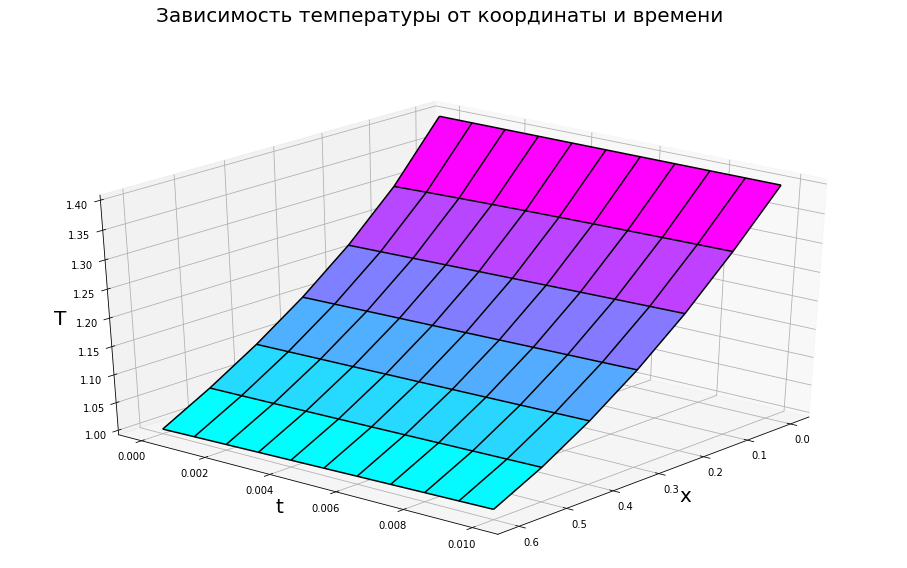
\includegraphics[scale=0.55]{pic1.png}}
		\label{pic1}
		\caption{}
	\end{figure}
	
	\newpage
	
	Изобразим проекции решения на плоскости $t=0, \; t=0.003, \; t=0.007, \; t=0.01$:
	
	\begin{figure}[h]
		\center{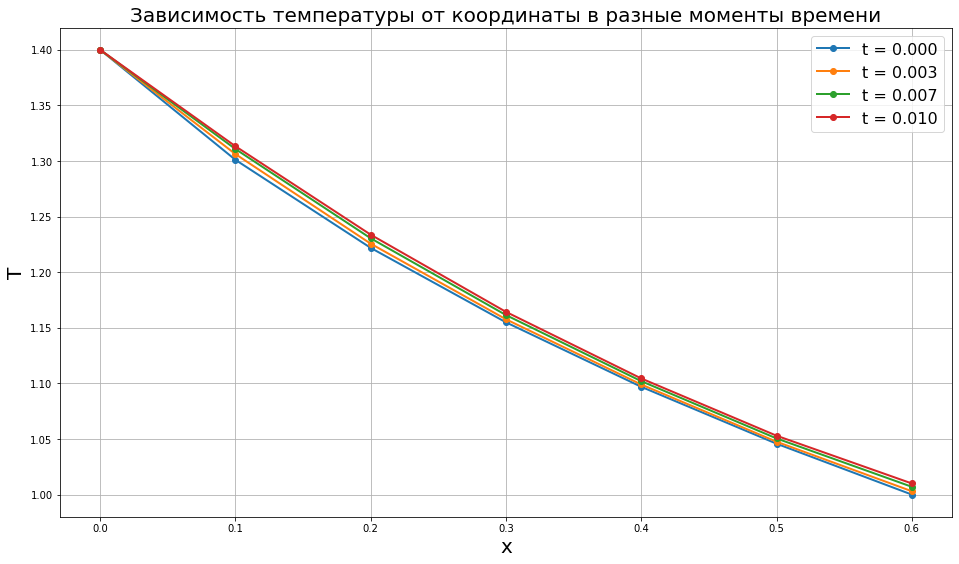
\includegraphics[scale=0.5]{pic2.png}}
		\label{pic2}
		\caption{}
	\end{figure}
	
	\newpage
	
	\section{Приложение}
	
	Табличное представление полученного решения:
	
	\begin{figure}[h]
		\center{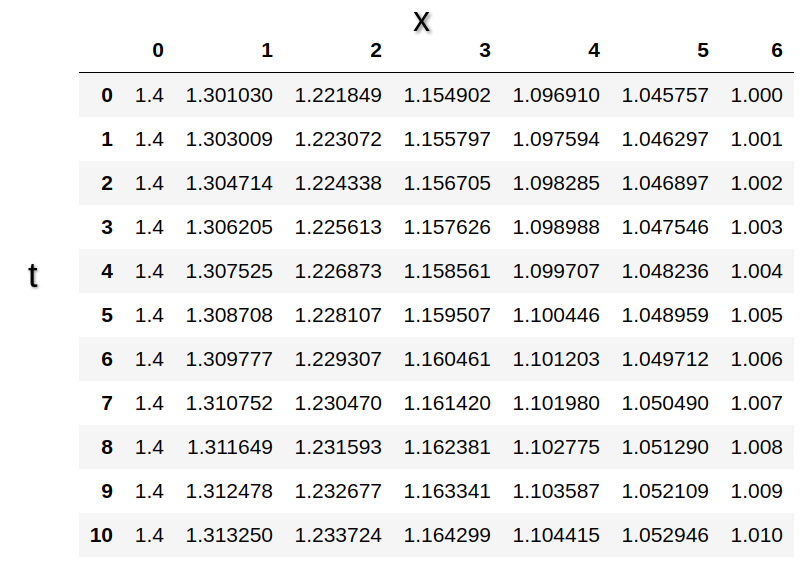
\includegraphics[scale=0.5]{pic3.png}}
		\label{pic3}
		\caption{}
	\end{figure}
	
	Далее представлен код программы на Python: \\
	
	\lstinputlisting[language=Python]{code.py}
	
\end{document}